\documentclass{article}

\usepackage[spanish,activeacute]{babel}
\usepackage{amsfonts}
\usepackage{graphicx}


\title{Taller 1}
\author{Mónica López Pola}

\begin{document}

\maketitle

\section*{Apartado 1}
$M = (\{q_0, q_1, q_3\}, \{a, b\}, \delta, q_0, \{q_2\})$

\section*{Apartado 2}
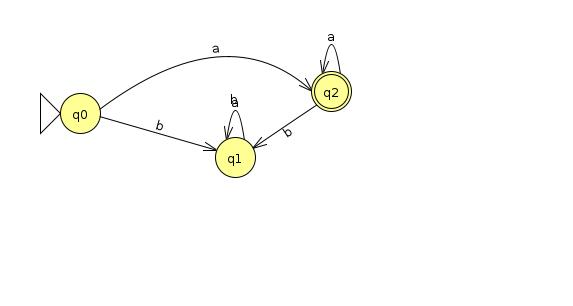
\includegraphics{as}

\section*{Apartado 3}
\begin{verbatim*}
{
  "name" : "a*bb*aa*",
  "representation" : {
    "K" : ["q0", "q1", "q2"],
    "A" : ["a", "b"],
    "s" : "q0",
    "F" : ["q2"],
    "t" : [["q0", "a", "q2"],
           ["q0", "b", "q1"],
           ["q1", "a", "q1"],
           ["q1", "b", "q1"],
           ["q2", "a", "q2"],
           ["q2", "b", "q1"]]
    }
}
\end{verbatim*}

\end{document}